\documentclass[main.tex]{subfiles}

\title{Glasser's Master Theorem}
\author{Senan Sekhon}
\date{\DTMToday}
% Created December 9, 2022

\begin{document}

\maketitle

\newtcolorbox{diagrambox}[1]{
    enhanced,
    colback=gray!5, colframe=black,
    segmentation style=solid,
    center upper,
    title={#1}, fonttitle=\large\sffamily\bfseries, center title,
}

\begin{definition}
    A function $f:\R\to\R$ \textbf{preserves the Lebesgue measure on $\R$} if for every Lebesgue measurable $A\sub\R$, we have $\mu(f^{-1}(A))=\mu(A)$, where $f^{-1}(A)=\{x\in\R\mid f(x)\in A\}$ is the pre-image of $A$ under $f$.
\end{definition}
\begin{examples}\leavevmode
    \begin{enumerate}
        \item For any $a\in\R$, the function $f(x)=x+a$ preserves the Lebesgue measure on $\R$.
        \item The function $f(x)=2x+\floor{x}-\floor{2x}$ preserves the Lebesgue measure on $\R$. This is because for each $n\in\Z$, the interval $[n,n+1)$ is mapped to two copies of itself, each with a slope of $2$ (so the pre-image of any subinterval of $[n,n+1)$ is mapped to two subintervals, each with half the length). Likewise, for any $m\in\Z\exc\{0\}$, the function $f(x)=mx+\floor{x}-\floor{mx}$ preserves the Lebesgue measure on $\R$.
    \end{enumerate}
\end{examples}

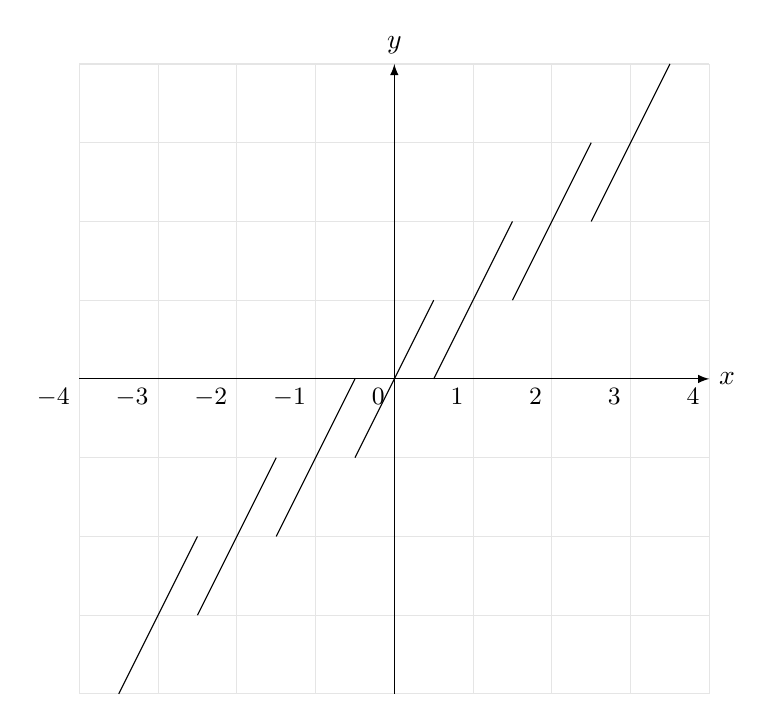
\begin{tikzpicture}
    \draw[thin, gray!20] (-4,-4) grid (4,4);
    \foreach \x in {-4,-3,...,4}
    \node[below left, font=\small] at (\x,0) {$\x$};
    \draw[-latex] (-4,0) -- (4,0) node[right]{$x$};
    \draw[-latex] (0,-4) -- (0,4) node[above]{$y$};
    \foreach \n in {-3,-2,...,3}
    \draw (\n-0.5,\n-1) --++ (1,2);
    
\end{tikzpicture}

\section{The Cauchy-Schlömilch Transformation}

\begin{lemma}[Cauchy-Schlömilch Transformation]\label{cauchy_schlomilch_transformation}
    Suppose $c>0$ and define $f:\R\exc\{0\}\to\R$ as follows:
    \begin{equation*}
        f(x) = x-\frac{c}{x}
    \end{equation*}
    Then $f$ preserves the Lebesgue measure on $\R$.
\end{lemma}
\begin{proof}
    Suppose $t\in\R$. We first solve the inequality $f(x)<t$, i.e. $x-\frac{c}{x}<t$.
    \begin{itemize}
        \item If $x>0$, this implies $x^2-tx-c<0$, and so $\frac{t-\sqrt{t^2+4c}}{2}<x<\frac{t+\sqrt{t^2+4c}}{2}$. Since $\frac{t-\sqrt{t^2+4c}}{2}<0$, this simplifies to $0<x<\frac{t+\sqrt{t^2+4c}}{2}$.
        \item If $x<0$, this implies $x^2-tx-c>0$, and so $x<\frac{t-\sqrt{t^2+4c}}{2}$ or $x>\frac{t+\sqrt{t^2+4c}}{2}$. Since $\frac{t+\sqrt{t^2+4c}}{2}>0$, this simplifies to $x<\frac{t-\sqrt{t^2+4c}}{2}$.
    \end{itemize}
    All in all, we have:
    \begin{equation*}
        f(x)<t \iff x<\frac{t-\sqrt{t^2+4c}}{2} \text{ or } 0<x<\frac{t+\sqrt{t^2+4c}}{2}
    \end{equation*}
    Similarly:
    \begin{equation*}
        f(x)>t \iff \frac{t-\sqrt{t^2+4c}}{2}<x<0 \text{ or } x>\frac{t+\sqrt{t^2+4c}}{2}
    \end{equation*}
    Note that for all $t\in\R$, we have:
    \begin{equation*}
        \pdv{t}\qty(\frac{t\pm\sqrt{t^2+4c}}{2})
        = \frac{1}{2} \pm \frac{t}{2\sqrt{t^2+4c}}
        \ge \frac{1}{2} - \frac{\abs{t}}{2\sqrt{t^2+4c}}
        > \frac{1}{2}-\frac{1}{2}
        = 0
    \end{equation*}
    Thus the functions $t\mapsto\frac{t\pm\sqrt{t^2+4c}}{2}$ are both strictly increasing in $t$.
    
    Now suppose $\alpha,\beta\in\R$, $\alpha<\beta$. Then we have:
    \begin{align*}
        \alpha<f(x)<\beta
        &\iff \qty(x<\frac{\beta-\sqrt{\beta^2+4c}}{2} \text{ or } 0<x<\frac{\beta+\sqrt{\beta^2+4c}}{2}) \\
        &\qquad \text{ and }\qty(\frac{\alpha-\sqrt{\alpha^2+4c}}{2}<x<0 \text{ or } x>\frac{\alpha+\sqrt{\alpha^2+4c}}{2})
    \end{align*}
    This reduces to:
    \begin{equation*}
        \frac{\alpha-\sqrt{\alpha^2+4c}}{2}<x<\frac{\beta-\sqrt{\beta^2+4c}}{2}
        \text{ or }
        \frac{\alpha+\sqrt{\alpha^2+4c}}{2}<x<\frac{\beta+\sqrt{\beta^2+4c}}{2}
    \end{equation*}
    The union of these intervals has length:
    \begin{equation*}
        \frac{\beta-\sqrt{\beta^2+4c}}{2}-\frac{\alpha-\sqrt{\alpha^2+4c}}{2}+\frac{\beta+\sqrt{\beta^2+4c}}{2}-\frac{\alpha+\sqrt{\alpha^2+4c}}{2}
        = \frac{\beta}{2}-\frac{\alpha}{2}+\frac{\beta}{2}-\frac{\alpha}{2}
        = \beta-\alpha
    \end{equation*}
    Thus $\mu(f^{-1}((\alpha,\beta)))=\mu((\alpha,\beta))$ for all $\alpha,\beta\in\R$, $\alpha<\beta$. By the \href{https://en.wikipedia.org/wiki/Carath%C3%A9odory%27s_extension_theorem}{Carathéodory extension theorem}, we have $\mu(f^{-1}(A))=\mu(A)$ for every Lebesgue measurable $A\sub\R$. Thus $f$ preserves the Lebesgue measure on $\R$.
\end{proof}

\begin{diagrambox}{Cauchy-Schlömilch Transformation}
    \pgfmathsetmacro{\c}{2}
    \pgfmathsetmacro{\a}{-3}
    \pgfmathsetmacro{\b}{-1}
    \pgfmathsetmacro{\negleft}{(\a-sqrt((\a)^2+4*\c))/2}
    \pgfmathsetmacro{\negright}{(\b-sqrt((\b)^2+4*\c))/2}
    \pgfmathsetmacro{\posleft}{(\a+sqrt((\a)^2+4*\c))/2}
    \pgfmathsetmacro{\posright}{(\b+sqrt((\b)^2+4*\c))/2}
    \pgfmathdeclarefunction{f}{1}{\pgfmathparse{#1-\c/#1}}
    
    \begin{tikzpicture}
        \draw[-latex] (-4,0) -- (4,0) node[right]{$x$};
        \draw[-latex] (0,-4) -- (0,4) node[right]{$y$};
        % \clip (-4,-4) rectangle (4,4);
        \draw[thick, smooth, color=blue, domain=-4:{2-sqrt(\c+4)}, samples=200] plot (\x,{f(\x)});
        \draw[thick, smooth, color=blue, domain={sqrt(\c+4)-2}:4, samples=200] plot (\x,{f(\x)});
        
        \fill[Orchid, fill opacity=0.2] (\negleft,\a) plot[domain=\negleft:\negright] (\x,{f(\x)}) -- (\negright,0) -- (\negleft,0) -- cycle;
        \fill[Orchid, fill opacity=0.2] (\posleft,\a) plot[domain=\posleft:\posright] (\x,{f(\x)}) -- (\posright,0) -- (\posleft,0) -- cycle;
        \fill[LimeGreen, fill opacity=0.2] (\negleft,\a) plot[domain=\negleft:\negright] (\x,{f(\x)}) -- (0,\b) -- (0,\a) -- cycle;
        \fill[LimeGreen, fill opacity=0.2] (\posleft,\a) plot[domain=\posleft:\posright] (\x,{f(\x)}) -- (0,\b) -- (0,\a) -- cycle;
    
        \draw[dashed] (\negleft,0) -- (\negleft,\a) -- (\posleft,\a) -- (\posleft,0);
        \draw[dashed] (\negright,0) -- (\negright,\b) -- (\posright,\b) -- (\posright,0);
        
        \draw[(-), very thick, Red] (\negleft,0) -- (\negright,0) node[midway, above=2pt]{$\Js_-$};
        \draw[(-), very thick, Red] (\posleft,0) -- (\posright,0) node[midway, above=2pt]{$\Js_+$};
        \draw[(-), very thick, Green] (0,\a) -- (0,\b) node[midway, left]{$\Is$};
    
        \node[blue] at (2,2.8) {$f(x)=x-\dfrac{c}{x}$};
        \node at (2.4,-2.4) {$\ell(\Is)=\ell(\Js_-)+\ell(\Js_+)$};
    \end{tikzpicture}
    
    For any interval on the $y$-axis, the length of the interval is equal to the sum of the lengths of the corresponding intervals on the $x$-axis.
\end{diagrambox}

\section{Glasser's Master Theorem}

The following theorem was first stated in 1983 by \href{https://wikitia.com/wiki/M._Lawrence_Glasser}{M. Lawrence Glasser} (1933--).

\begin{theorem}[Glasser's Master Theorem]\label{glassers_master_theorem}
    Suppose $a_1,a_2,\cdots,a_n\in\R$, $c_1,c_2,\ldots,c_n>0$ and $b\in\R$. Define $f:\R\exc\{a_1,a_2,\ldots,a_n\}$ as follows:
    \begin{equation*}
        f(x) = x-b-\frac{c_1}{x-a_1}-\frac{c_2}{x-a_2}-\cdots-\frac{c_n}{x-a_n}
    \end{equation*}
    Then $f$ preserves the Lebesgue measure on $\R$.
\end{theorem}
\begin{proof}
    Assume without loss of generality that $a_1<a_2<\cdots<a_n$. Define $a_0=-\infty$ and $a_{n+1}=\infty$, and for each $k\in\{0,1,\ldots,n\}$, define $I_k=\qty(a_k,a_{k+1})$. Note that for all $x\in\R\exc\{a_1,a_2,\ldots,a_n\}$, we have:
    \begin{equation*}
        f'(x)
        = 1+\frac{c_1}{(x-a_1)^2}+\frac{c_2}{(x-a_2)^2}+\cdots+\frac{c_n}{(x-a_n)^2}
        > 1
    \end{equation*}
    We also have $\lim_{x\to a_k^-} f(x)=\infty$ and $\lim_{x\to a_k^+}=-\infty$ for all $k\in\{0,1,\ldots,n\}$. Thus for each $k\in\{0,1,\ldots,n\}$, the restriction of $f$ to $I_k$ is a bijection from $I_k$ to $\R$.\\

    Define $g_k:\R\to I_k$ as the inverse of the restriction of $f$ to $I_k$. Then for each $y\in\R$, the equation $f(x)=y$ has exactly $n+1$ solutions, namely $g_0(y),g_1(y),\ldots,g_n(y)$. Multiplying both sides of $f(x)-y=0$ by $(x-a_1)(x-a_2)\cdots(x-a_n)$, we get:
    \begin{align*}
        (x-a_1)(x-a_2)\cdots(x-a_n)\qty(x-b-\frac{c_1}{x-a_1}-\frac{c_2}{x-a_2}-\cdots-\frac{c_n}{x-a_n}) &= 0 \\
        (x-a_1)(x-a_2)\cdots(x-a_n)(x-b-y) + P_{n-1}(x) &= 0
    \end{align*}
    Where $P_{n-1}(x)$ is a polynomial in $x$ of degree at most $n-1$. Since the left side is a monic polynomial of degree $n+1$ that vanishes at $g_0(y),g_1(y),\ldots,g_n(y)$, it must be equal to $(x-g_0(y))(x-g_1(y))\cdots(x-g_n(y))$. Thus we have:
    \begin{equation*}
        (x-a_1)(x-a_2)\cdots(x-a_n)(x-b-y) + P_{n-1}(x)
        = (x-g_0(y))(x-g_1(y))\cdots(x-g_n(y))
    \end{equation*}
    Comparing the coefficients of $x^n$ on each side, we get:
    \begin{equation*}
        -(a_1+a_2+\cdots+a_n+b+y) = -(g_0(y)+g_1(y)+\cdots+g_n(y))
    \end{equation*}
    Since each $g_k$ is strictly increasing, for any $y,z\in\R$, $y<z$, we have $f(x)\in(y,z)$ if and only if $x\in(g_k(y),g_k(z))$ for some $k\in\{0,1,\ldots,n\}$. This yields:
    \begin{align*}
        \mu(f^{-1}((y,z)))
        &= \mu\qty(\kupp_{k=0}^n (g_k(y),g_k(z))) \\
        &= \sum_{k=0}^n \mu((g_k(y),g_k(z))) \\
        &= \sum_{k=0}^n (g_k(z)-g_k(y)) \\
        &= (a_1+a_2+\cdots+a_n+b+z)-(a_1+a_2+\cdots+a_n+b+y) \\
        &= z-y \\
        &= \mu((y,z))
    \end{align*}
    Thus $\mu(f^{-1}((y,z)))=\mu((y,z))$ for all $y,z\in\R$, $y<z$. By the \href{https://en.wikipedia.org/wiki/Carath%C3%A9odory%27s_extension_theorem}{Carathéodory extension theorem}, we have $\mu(f^{-1}(A))=\mu(A)$ for every Lebesgue measurable $A\sub\R$. Thus $f$ preserves the Lebesgue measure on $\R$.
\end{proof}
\begin{remark}
    If $n=1$, i.e. $f(x)=x-b-\frac{c}{x-a}$ (where $c>0$), we can explicitly compute the inverse of $f$:
    \begin{equation*}
        f^{-1}(y) = \frac{y+b+a\pm\sqrt{(y+b-a)^2+4c}}{2}
    \end{equation*}
    The $\pm$ corresponds to the fact that there are two values of $x$ for each value of $y$, one with $x>b$ and one with $x<b$.
\end{remark}

\begin{theorem}
    Suppose $f:\R\to\R$ preserves the Lebesgue measure on $\R$. Then for any $\phi\in L^1(\R)$, we have:
    \begin{equation*}
        \int_{\R} \phi(f(x))\dmu(x) = \int_{\R} \phi(x)\dmu(x)
    \end{equation*}
\end{theorem}
\begin{proof}
    If $\phi=1_A$ is an indicator function of some Lebesgue measurable $A\sub\R$, this reduces to $\mu(f^{-1}(A))=\mu(A)$, which is true as $f$ preserves the Lebesgue measure on $\R$ by assumption. By linearity, the result holds for simple functions (linear combinations of indicator functions), and by approximation, it holds for all integrable functions.

    \begin{equation*}
        \int_{\R} \phi(f(x))\dmu(x)
    \end{equation*}
\end{proof}

In the case of $f(x)=x-\frac{c}{x}$ (the Cauchy-Schlömilch transformation), we can give a much simpler proof:

\begin{proof}
    Substituting $u=-\frac{c}{x}$, we get:
    \begin{equation*}
        \int_{-\infty}^{\infty} \phi\qty(x-\frac{c}{x})\dx
        = c\int_{-\infty}^{\infty} \frac{1}{u^2}\phi\qty(u-\frac{c}{u})\du
    \end{equation*}
    We now add the left side of the above equation to both sides:
    \begin{align*}
        2\int_{-\infty}^{\infty} \phi\qty(x-\frac{c}{x})\dx
        &= \int_{-\infty}^{\infty} \phi\qty(x-\frac{c}{x})\dx
        + c\int_{-\infty}^{\infty} \frac{1}{x^2}\phi\qty(x-\frac{c}{x})\dx \\
        &= \int_{-\infty}^{\infty} \qty(1+\frac{c}{x^2})\phi\qty(x-\frac{c}{x})\dx
    \end{align*}
    We now substitute $y=x-\frac{c}{x}$. Note that as $x$ runs from $-\infty$ to $\infty$, $y$ runs from $-\infty$ to $\infty$ \emph{twice} (once when $x<0$ and once when $x>0$). This introduces a factor of $2$ below:
    \begin{equation*}
        2\int_{-\infty}^{\infty} \phi\qty(x-\frac{c}{x})\dx
        = 2\int_{-\infty}^{\infty} \phi(y)\dy
    \end{equation*}
    Dividing by $2$ yields the desired result.
\end{proof}

\begin{example}
    \begin{equation*}
        \int_{-\infty}^{\infty} \frac{x^2}{x^4+1}\dx
        = \int_{-\infty}^{\infty} \frac{1}{\qty(x-\frac{1}{x})^2+2}\dx
        = \int_{-\infty}^{\infty} \frac{1}{x^2+2}\dx
        = \frac{\pi}{\sqrt{2}}
    \end{equation*}
\end{example}

\begin{example}
    Unfortunately, $\frac{1}{x^4+1}$ does not have a simple expression in terms of $x-\frac{1}{x}$. However, note that:
    \begin{equation*}
        \frac{x^2+1}{x^4+1}
        = \frac{1+\frac{1}{x^2}}{\qty(x-\frac{1}{x})^2+2}
    \end{equation*}
    This allows us to easily find $\int_{-\infty}^{\infty} \frac{x^2+1}{x^4+1}\dx$. Note that we are \emph{not} using \hyperref[glassers_master_theorem]{Glasser's master theorem} here, we are simply substituting $u=x-\frac{1}{x}$.
    \begin{equation*}
        \int_{-\infty}^{\infty} \frac{x^2+1}{x^4+1}\dx
        = \int_{-\infty}^{\infty} \frac{1+\frac{1}{x^2}}{\qty(x-\frac{1}{x})^2+2}\dx
        = 2\int_{-\infty}^{\infty} \frac{1}{u^2+2}\du
        = 2\qty(\frac{\pi}{\sqrt{2}})
        = \sqrt{2}\pi
    \end{equation*}
    The factor of $2$ comes from the fact that as $x$ runs from $-\infty$ to $\infty$, $u$ runs from $-\infty$ to $\infty$ twice. Thus, we have:
    \begin{equation*}
        \int_{-\infty}^{\infty} \frac{1}{x^4+1}\dx
        = \int_{-\infty}^{\infty} \frac{x^2+1}{x^4+1}\dx - \int_{-\infty}^{\infty} \frac{x^2}{x^4+1}\dx
        = \sqrt{2}\pi - \frac{\pi}{\sqrt{2}}
        = \frac{\pi}{\sqrt{2}}
    \end{equation*}
\end{example}

\begin{example}
    \begin{equation*}
        \int_{-\infty}^{\infty} \frac{x^4}{x^8+1}\dx
        = \int_{-\infty}^{\infty} \frac{1}{\qty(x-\frac{1}{x})^4+4\qty(x-\frac{1}{x})^2+2}\dx
        = \int_{-\infty}^{\infty} \frac{1}{x^4+4x^2+2}\dx
        = \frac{\sqrt{4-2\sqrt{2}}}{4}\pi
    \end{equation*}
    \begin{equation*}
        \int_{-\infty}^{\infty} \frac{x^4}{x^8+x^4+1}\dx
        = \int_{-\infty}^{\infty} \frac{1}{\qty(x-\frac{1}{x})^4+4\qty(x-\frac{1}{x})^2+3}\dx
        = \int_{-\infty}^{\infty} \frac{1}{x^4+4x^2+3}\dx
        = \frac{3-\sqrt{3}}{6}\pi
    \end{equation*}
    \begin{equation*}
        \int_{-\infty}^{\infty} \frac{x^4}{x^8+ax^4+1}\dx
        = \int_{-\infty}^{\infty} \frac{1}{\qty(x-\frac{1}{x})^4+4\qty(x-\frac{1}{x})^2+a+2}\dx
        = \int_{-\infty}^{\infty} \frac{1}{x^4+4x^2+a+2}\dx
        = \sqrt{\frac{\sqrt{a+2}-2}{2(a^2-4)}}\pi
    \end{equation*}
    \begin{equation*}
        \int_{-\infty}^{\infty} \frac{x^6+x^4}{x^{10}+1}\dx
        = \int_{-\infty}^{\infty} \frac{1}{\qty(x-\frac{1}{x})^4+3\qty(x-\frac{1}{x})^2+1}\dx
        = \int_{-\infty}^{\infty} \frac{1}{x^4+3x^2+1}\dx
        = \frac{\pi}{\sqrt{5}}
    \end{equation*}
    \begin{equation*}
        \int_{-\infty}^{\infty} \frac{x^4}{(x^4+1)(x^4-x^2+1)}\dx
        = \int_{-\infty}^{\infty} \frac{1}{\qty(x-\frac{1}{x})^4+3\qty(x-\frac{1}{x})^2+2}\dx
        = \int_{-\infty}^{\infty} \frac{1}{x^4+3x^2+2}\dx
        = \qty(1-\frac{1}{\sqrt{2}})\pi
    \end{equation*}
\end{example}

\begin{example}
    \begin{equation*}
        \int_{-\infty}^{\infty} e^{-\qty(x-\frac{1}{x})^2}\dx
        = \int_{-\infty}^{\infty} e^{-x^2}\dx
        = \sqrt{\pi}
    \end{equation*}
\end{example}
\begin{example}
    \begin{equation*}
        \int_{-\infty}^{\infty} \sech(x-\frac{1}{x})\dx
        = \int_{-\infty}^{\infty} \sech(x)\dx
        = \pi
    \end{equation*}
\end{example}

\section{Generalization to infinitely many poles}

We can generalize \hyperref[glassers_master_theorem]{Glasser's master theorem} to more exotic functions.

\begin{diagrambox}{The function $f(x)=x-\cot(x)$}
    \pgfmathdeclarefunction{f}{1}{\pgfmathparse{#1-cot(180*#1)}}
    
    \begin{tikzpicture}
        \draw[-latex] (-4,0) -- (4,0) node[right]{$x$};
        \draw[-latex] (0,-4) -- (0,4) node[right]{$y$};
        \clip (-4,-4) rectangle (4,4);
        \foreach \n in {-4,-3,...,3}
            \draw[thick, smooth, color=blue, domain={\n+0.01}:{\n+0.99}, samples=200] plot (\x,{f(\x)});
        
        % \fill[Orchid, fill opacity=0.2] (\negleft,\a) plot[domain=\negleft:\negright] (\x,{f(\x)}) -- (\negright,0) -- (\negleft,0) -- cycle;
        % \fill[Orchid, fill opacity=0.2] (\posleft,\a) plot[domain=\posleft:\posright] (\x,{f(\x)}) -- (\posright,0) -- (\posleft,0) -- cycle;
        % \fill[LimeGreen, fill opacity=0.2] (\negleft,\a) plot[domain=\negleft:\negright] (\x,{f(\x)}) -- (0,\b) -- (0,\a) -- cycle;
        % \fill[LimeGreen, fill opacity=0.2] (\posleft,\a) plot[domain=\posleft:\posright] (\x,{f(\x)}) -- (0,\b) -- (0,\a) -- cycle;
    
        % \draw[dashed] (\negleft,0) -- (\negleft,\a) -- (\posleft,\a) -- (\posleft,0);
        % \draw[dashed] (\negright,0) -- (\negright,\b) -- (\posright,\b) -- (\posright,0);
        
        % \draw[(-), very thick, Red] (\negleft,0) -- (\negright,0) node[midway, above=2pt]{$\Js_-$};
        % \draw[(-), very thick, Red] (\posleft,0) -- (\posright,0) node[midway, above=2pt]{$\Js_+$};
        % \draw[(-), very thick, Green] (0,\a) -- (0,\b) node[midway, left]{$\Is$};
    
        % \node[blue] at (2,2.8) {$f(x)=x-\dfrac{c}{x}$};
        % \node at (2.4,-2.4) {$\ell(\Is)=\ell(\Js_-)+\ell(\Js_+)$};
    \end{tikzpicture}
    
    The function $f:\R\exc\pi\Z\to\R$, $f(x)=x-\cot(x)$ is qualitatively very similar to the functions in \hyperref[glassers_master_theorem]{Glasser's master theorem} (except that this function has \emph{infinitely} many poles).
\end{diagrambox}

It turns out that $f$ also preserves the Lebesgue measure on $\R$. This is because:
\begin{equation*}
    \cot(x) = \cdots + \frac{1}{x-3\pi} + \frac{1}{x-2\pi} + \frac{1}{x-\pi} + \frac{1}{x} + \frac{1}{x+\pi} + \frac{1}{x+2\pi} + \frac{1}{x+3\pi} + \cdots
\end{equation*}
More formally, for all $x\in\R\exc\pi\Z$, we have:
\begin{equation*}
    \cot(x) = \limn\sum_{k=-n}^n \frac{1}{x+k\pi}
\end{equation*}
\url{https://math.stackexchange.com/a/1015739}


There are many more functions that preserve the Lebesgue measure on $\R$. The example below is continuous and piecewise linear.

\begin{example}
    Define $f:\R\to\R$ as follows:
    \begin{center}
        \begin{tikzpicture}
            \begin{scope}[scale=0.5, every node/.style={transform shape, scale=2, color=black}]
                \draw[-latex] (-5,0) -- (5,0);
                \draw[-latex] (0,-5) -- (0,5);
                \draw[thick, blue] (-5,-5) -- (-3,-3) node[below right]{$(-3,-3)$} -- (-1,3) node[above left]{$(-1,3)$} -- (1,-3) node[below right]{$(1,-3)$} -- (3,3) node[above left]{$(3,3)$} -- (5,5);
                \foreach \x/\y in {-3/-3,-1/3,1/-3,3/3}
                    \fill (\x,\y) circle (4pt);
            \end{scope}
            \node at (-6,0) {
                $f(x) = \begin{cases}
                    x & x<-3 \text{ or } x>3 \\
                    3x+6 & -3<x<-1 \\
                    -3x & -1\le x\le 1 \\
                    3x-6 & 1<x<3
                \end{cases}$
            };
        \end{tikzpicture}
    \end{center}
    Then $f$ is continuous, piecewise linear and preserves the Lebesgue measure on $\R$. Informally, this is because $f(x)=x$ except on $(-3,3)$, where it traverses the interval $(-3,3)$ three times, each with a slope of $\pm 3$. More examples can be constructed similarly, e.g. by traversing an interval $5$ times, each with a slope of $\pm 5$.
\end{example}

\end{document}